\documentclass[oneside,numberorder]{csbachelor}
% \documentclass[twoside,authoryear]{csbachelor}
%==============================================================
%==============================================================

\usepackage{url}
\usepackage{subfigure}

% 张海:其他引用
\usepackage[hidelinks]{hyperref}
\usepackage{pdfpages}

% 一些全局工具的定义
\DeclareMathOperator*{\argmin}{arg\,min}
\DeclareMathOperator*{\argmax}{arg\,max}

%==============================================================
%==============================================================

\begin{document}

\pagestyle{empty}

%==============================================================
%==============================================================

% 论文题目:{中文}{英文}
\zjutitle{深度行人再识别学习}
{Deep Person Re-Identification Learning}
% 作者:{中文姓名}{英文}{学号}
\zjuauthor{王兴路}{Xinglu Wang}{3140102282}
% 指导教师:{导师中文名}{导师英文名}
\zjumentor{李英明}{Yingming Li}
% 个人信息:{年级}{专业名称}
\zjuinfo{2014级}{信息工程}
% 学院信息:{学院中文}{学院英文}
\zjucollege{信息与电子工程学院}{College of Information Science \& Electronic Engineering}
% 日期:{Submitted Date}
%\zjudate{2018-02-25}

%==============================================================

{  \thispagestyle{empty}

{
\setlength{\parindent}{0em}
\renewcommand{\baselinestretch}{2}

\vspace*{-7mm}

\begin{center}
  \includegraphics[width=108mm]{data/cover/xiaoming}
\end{center}

\vspace{-1mm}

{
\renewcommand{\baselinestretch}{1.8}
\heiti\erhao\bfseries
\centering
本~~科~~生~~毕~~业~~设~~计 \\
文献综述和开题报告 \par
}

\vspace{4em}

\begin{center}
  \includegraphics[width=35mm]{data/cover/xiaobiao}
\end{center}

\vspace{3em}

{
	\renewcommand{\baselinestretch}{1.65}
	\sanhao
	\centering
	{\kaiti\bfseries 姓名与学号} \; \underline{\makebox[13em]{\songti\zjuauthornamec~~\zjuauthorid}} \\ \vspace{0.9em}
	{\kaiti\bfseries 指导教师} \; \underline{\makebox[14em]{\songti\zjumentorc}} \\ \vspace{0.9em}
	{\kaiti\bfseries 年级与专业} \; \underline{\makebox[13em]{\songti\zjugrade~~\zjumajor}} \\ \vspace{0.9em}
	{\kaiti\bfseries 所在学院} \; \underline{\makebox[14em]{\songti\zjucollegec}} \par
}
}

\ifthenelse{\equal{\zjuside}{T}}{\newpage\mbox{}\thispagestyle{empty}}{}
 }

{  \newpage

\thispagestyle{empty}

{
\setlength{\parindent}{0em}
\renewcommand{\baselinestretch}{2}
{\songti\sihao\bfseries

一、 \; 题目: \; \underline{\makebox[24em]{\zjutitlec}}

\vspace{2em}

二、 \; 指导教师对文献综述和开题报告的具体内容要求: \\ \par
}
{
  \songti\xiaosi 

% 多个摄像头下的行人再识别是一个非常挑战的问题,尤其是摄像头之间没有交叉视野的情况下。现有的算法主要集中在使用相同的深度神经网络对输入的不同视角下的图像或视频对,进行特征学习,然后通过距离度量,确定是否代表同一个人。但是,一方面由于受到标注数据集有限的影响,算法的性能会受到影响;另一方面,现有的算法不能很好的利用图像和视频数据的特征多样性,提升算法的鲁棒性。 研究内容:在本次毕业论文中,一方面,我们计划引入生成对抗的思想,通过产生逼真的假样本,对训练的样本集进行扩充,提高算法的总体性能;另一方面,利用多种深度网络构建多种特征来学习样本之间的相似性,增强算法的鲁棒性。 具体要求:学会分析图像视频数据,构建新颖的模型,解决现有算法的不足,争取发表一篇高水平学术论文。

文献综述的主要目的是为论文的写作和研究方法提供支持, 进而表明本研究是有价值的。具体要求归纳和总结国内外相关文献对该研究问题做过哪些方面的研究,取得了哪些阶段性的成果,以及既有研究中存在的一些难点和局限性。在进行文献综述时,不要只是简单罗列之前的研究成果,而是要紧扣自己的研究内容,对与自己要解决的具体研究问题紧密相关的文献进行必要的归纳、总结、批判并提出一些新的观点和可能的新研究方向。开题报告一般由以下几个方面组成:1)研究问题;2)研究目的和意义;3)文献综述;4)研究方法;5)论文的纲要;6)参考文献。
}

\vspace{9cm}
}

{
\songti\xiaosi\bfseries
\begin{flushright}
  指导教师(签名) \; \underline{\hspace{6em}} \\
  年 \qquad 月 \qquad 日
\end{flushright}
}

\ifthenelse{\equal{\zjuside}{T}}{\newpage\mbox{}\thispagestyle{empty}}{}
 }

{
\pagestyle{empty}
{
	\renewcommand{\thispagestyle}[1]{}
	\tableofcontents
}
\clearpage
\pagestyle{plain}
% \tableofcontents
% \thispagestyle{toc}
% \chaptermark{目录}
}

\mainmatter

{
	\pagestyle{kaitibaogao}
	\makeatletter
	\let\ps@plain\ps@kaitibaogao
	\makeatother
	\chapter{文献综述}

\section{背景介绍}

\indent 行人再识别(Person Re-identification,简称ReID), 也称行人重识别\cite{zheng2016person},如图~\ref{figure:background},是利用计算机视觉技术,在图像或者视频集合(gallery)中找到与询问图片(query)相似行人的任务。理论上来说,视频监控中的行人再识别系统应该被分解为三个子模块:行人检测、行人跟踪、行人检索。前两个模块是计算机视觉中已经存在的任务,因此大多研究者所指的行人再识别问题着力解决行人检索问题\cite{zheng2017person}。本文也不例外,着力解决光照、姿态、视角急剧变化下的行人再识别/检索问题。

\begin{figure}[!htbp]
    \centering
    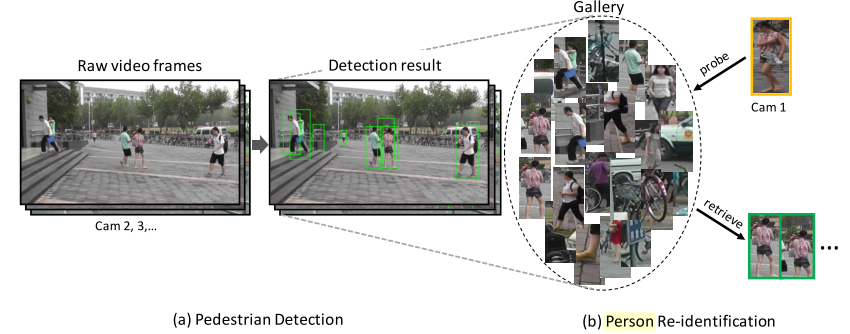
\includegraphics[width=\linewidth,keepaspectratio]{data/kaitibaogao/background.png}
    \caption{典型行人再识别系统的流程,整个行人再识别系统包括:视频行人检测、行人跟踪、行人检索。目前的工作主要集中在行人检索问题上。因此大多研究者所指的行人再识别问提指的是其中的子模块——行人检索问题。}
    \label{figure:background}
\end{figure}

行人再识别中存在许多挑战。由于行人的非刚性运动、检测器的误差、摄像头的视角变化,同一行人的不同图片往往存在严重的空间失配(Spatial Misalignment);行人没有可靠的生物特征,只能从属性、语义层面的特征加以区分;未标定的摄像机参数、巨大的时空跨度,这些都进一步增加了再识别的难度;同时现有的数据集规模相对较小,不存在ImageNet或者MegaFace这样的大规模、可以泛化迁移(Transfer)到任意子领域(domain)的数据集。这导致数据集间存在较大偏差(domain bias/domain shift),从一个数据集到另一个数据集,模型的性能通常都会下降。

\section{国内外研究现状}

由于行人再识别的应用和研究的价值,他在计算机视觉领域受到了越来越多的关注和巨大的发展。近几年,再识别领域投稿数量增加,性能也呈指数增长,2015年好的模型cmc-1(Cumulative Matching Characteristic)只有$65\%$。17年在$80\%-85\%$。但是在17年短短11月,Arxiv上公布的文章已经达到了$90\%-96\%$。18年行人再识别领域的cmc-1已经能够在大型数据集上超越人类的表现。
目前的研究者大多从几个固定的方面深入研究。从损失函数分类上看,行人再识别主要使用分类损失、度量损失,分别对应表征学习和度量学习。这是再识别的基本方法,在此基础上,国内外的研究者往往从特征学习、网络结构的设计(如引入结构先验——行人由几个部分构成、具有相对空间位置关系)或者提出新的问题(视频再识别、生成数据、大规模检索、弱监督学习)等方面着手。本综述也将从这些方面展开。

    \subsection{表征学习与度量学习}

    \textbf{表征学习(Representation learning):}通过转化为分类(Classification/ Identification)问题或者验证(Verification)问题,进行监督性学习训练,取全连接层的特征作为很好的表征。之所以说是很好的表征,是因为输入图片原本线性不可分,但是最后一层线性分类层的特征变得线性可分,从而使得后续任务变得简单。w无论是分类还是验证问题,在转化之后,会使用softmax作为激活函数。在有的论文中,作者认为光靠行人的ID信息不足以学习出一个泛化能力足够强的模型,于是额外标注了行人图片的属性特征,例如性别、头发、衣着等属性。通过引入行人属性标签,模型不但要准确地预测出行人ID,还要预测出各项正确的行人属性。

    \textbf{度量学习(Metric learning):}度量学习广泛应用于图像检索。不同于表征学习,度量学习通过设计距离度量函数,直接学习特征。优化目标直接就是同一行人不同图片特征之间的相似度更小,不同行人的更大。损失函数使得相同行人图片(正样本对)的距离尽可能小,不同行人图片(负样本对)的距离尽可能大。常用的度量学习损失方法有对比损失(Contrastive loss) \cite{varior2016gated}、三元组损失(Triplet loss)、四元组损失(Quadruplet loss)、难样本采样三元组损失(Triplet hard loss with batch hard mining, TriHard loss)\cite{hermans2017defense}、边界挖掘损失(Margin sample mining loss, MSML)

    两者最终学到的特征,都是语义上紧凑的表示,能够根据ID聚成不同的类别,有利于后续任务的进行。但是区别在于表征学习是通过定义其他有关联的分类任务间接学到表征的。

    \begin{figure}[!htbp]
        \centering
        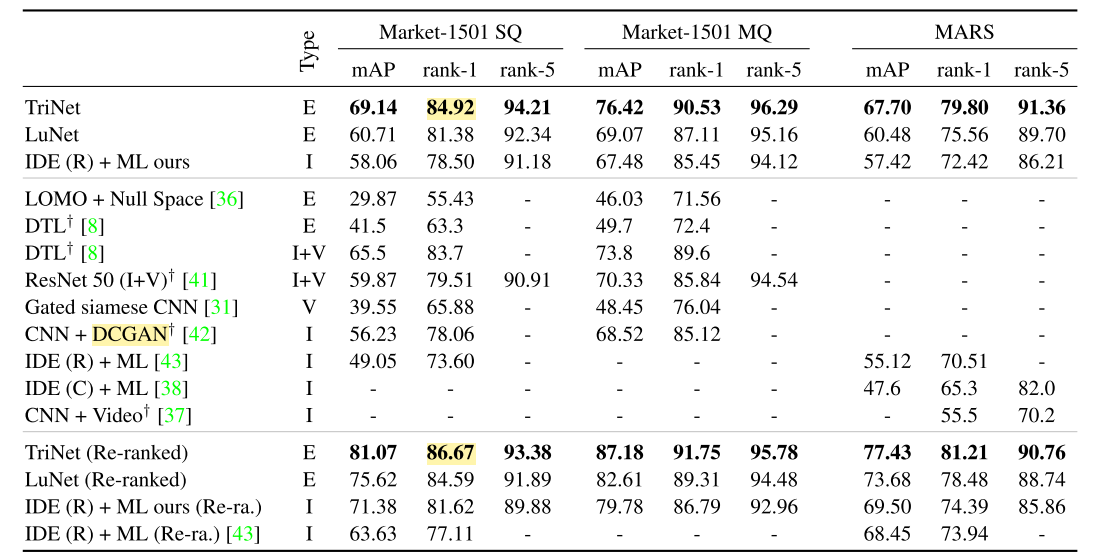
\includegraphics[width=\linewidth,keepaspectratio]{data/kaitibaogao/loss-perf.png}
        \caption{表示学习、度量学习的方法比较,其中,TriHard方法获得了最好的效果。在不使用Rerank后处理的情况下,得到了84.92的rank-1指标,在rerank和使用multi-shot查询的情况下,获得了91.75的rank-1指标。}
        \label{figure:loss}
    \end{figure}

    表征学习实现简单,当每个ID都有充足的训练图片时效果很有竞争力。如图~\ref{figure:loss},实践证明,在行人再识别、人脸验证这一类问题,度量学习只要训练得当,就能够获得更快的收敛速度与泛化能力。因此,本节将重点叙述表征学习的方法。

    对比损失用于训练孪生网络(Siamese network),网络含有两条分支,三元损失用于训练三条分支的网络。但是由于各条分支之间参数共享,所以可以使用一条分支高效实现。首先介绍对比损失,假设输入图像a和b,提取到的特征之间的距离定义为
    \begin{equation} {d_{a,b}} = \left\|{f_{{I_a}}} - {f_{{I_b}}}\right\|{^2}\end{equation} 
    
    当两张图属于同一行人时,标签y=1,不同行人时,标签y=0,则对比损失为
    \begin{equation} {L_c} = yd_{a,b}^2 + (1 - y)(\alpha  - {d_{a,b}})_+^2\end{equation} 
    
    三元损失的三个输入分别为锚定图片(Anchor) a ,正样本图片(Positive) p和负样本图片(Negative) n。图片 a 和图片 p 为一对正样本对,图片 a 和图片 n 为一对负样本对。三元组损失表示为:
    \begin{equation} {L_t} = {({d_{a,p}} - {d_{a,n}} + \alpha )_ + }\end{equation} 
    
    传统的三元组随机从训练数据中抽样三张图片,由于随机抽取的往往是无用信息,导致训练时间长、收敛慢,而且容易训练崩塌。因而长期以来,研究者普遍认为使用度量损失往往比表示学习中的分类验证损失效果差。\cite{liu2017quality}提出了一种基于训练批量(Batch)的在线难样本采样方法——TriHard Loss,比所有17年所有的最新方法性能和收敛速度都好了一大截。
    对于每一个训练batch,随机挑选 P 个ID的行人,每个行人随机挑选 K 张不同的图片,即一个batch含有 $P\times K$ 张图片。之后对于batch中的每一张图片 a ,我们可以挑选一个最难的正样本和一个最难的负样本和 a 组成一个三元组。

    我们定义和a 具有相同ID的图片集为 A,剩下不同ID的图片图片集为 B,则TriHard损失表示为:
    \begin{equation} 
        L_t=\frac{1}{PK}\sum_{a \in batch} \left( \max_{p \in A} d_{a,p} -  \min_{n \in B} d_{a,n} +\alpha \right)_+
    \end{equation}

    \subsection{融合局部特征}

    在行人再识别中,一个很热门的研究方向就是提取更好的局部特征\cite{reciprocal,liu2017hydraplus,zhao2017spindle,glad},18年性能很高的几篇论文基本上都使用了局部特征\cite{liu2017hydraplus,zhao2017spindle}。其中对齐再识别\cite{zhang2017align}使用最短路径自动匹配局部特征,算法复杂度较高,通过辅助全局特征的训练获得了超过人类的表现,详细可以参考文献翻译。

    上下文特征\cite{latent}使用STN结合先验定位可变性的行人部分,从原始图片中预测定位参数,从而便于后续的网络将注意力集中于具有潜在语义的身体部分。考虑到视频监控环境下行人的姿态先验——行人通常直立于地面,作者使用了4个自由度的仿射变换矩阵,建模了尺度、平移方面的可变性变换。
    \begin{equation} 
        \left(\begin{array}{c} 
        x^{in}_i \\
        y^{in}_i
        \end{array}\right) =\left[ \begin{array}{ccc}
        s_x & 0 & t_x \\
        0 & s_y & t_y
        \end{array}\right] \left(\begin{array}{c}
        x^{out}_{i} \\
        y^{out}_i \\
        1
        \end{array}\right)
    \end{equation}

    由于具有了可变性的特性,学到的身体部分能够减轻视角和背景带来的类内差异。但是由于随机生成的反射矩阵参数会产生巨大形变,作者不得不增加正则项将其限制于先验的附近。最终将全局特征与身体各部分的特征融合,结合分类损失训练。

    \subsection{GAN生成样本}

    如图~\ref{figure:dataset}所示,ReID有一个非常大的问题就是数据获取困难,截止CVPR18 deadline截稿之前,最大的ReID数据集只有1k ID,36k 图片。视频数据集的图片数量当然达到上万,但是冗余较高,有效的图片仍然少于几千张。因此,使用gan生成图片提升泛化能力显得非常重要。

    \begin{figure}[!htbp]
        \centering
        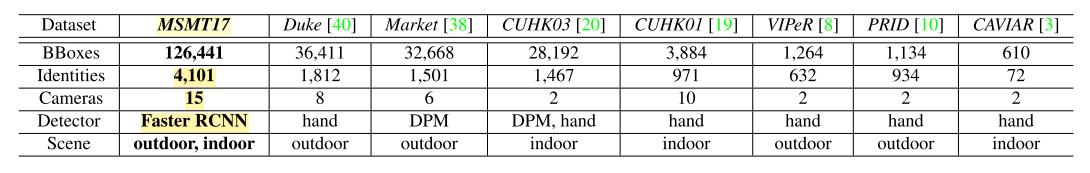
\includegraphics[width=\linewidth,keepaspectratio]{data/kaitibaogao/dataset.png}
        \caption{ReID常用数据集统计信息,可以看见,ReID领域公开数据集规模通常较小}
        \label{figure:dataset}
    \end{figure}

    试管实验一文\cite{zheng2017unlabeled}是第一篇用GAN做ReID的文章,由于生成的图像质量较差,没有明确的id信息,论文使用的是标签平滑的方法,将label vector每一个元素的值取为各个类别的均匀分布。生成的图像作为训练数据加入到训练之中,相当于在训练过程中引入了适当的噪声,避免了过拟合提升了泛化能力。
    
    在此基础上,姿态归一化一文\cite{qian2017pose}提出了改进,一方面能够相同ID的行人,另一方面克服了行人姿态不同带来的类内差异。

    \begin{figure}[!htbp]
        \centering
        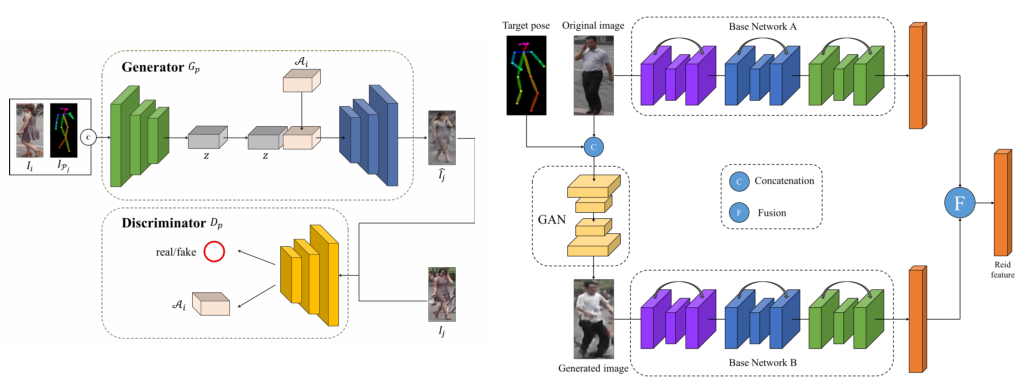
\includegraphics[width=\linewidth,keepaspectratio]{data/kaitibaogao/pose-norm.png}
        \caption{姿态归一化一文\cite{qian2017pose}所使用的网络结构。左图:最终网络结构——原始图片提取特征与姿态归一化后图片提取的特征融合,用于再识别。右图:生成姿态归一化图片的GAN网络结构,融合姿态、ID、属性等信息,生成较高质量的图片。}
        \label{figure:pose-norm}
    \end{figure}

    论文首先使用在coco上预训练的pose estimation网络提取骨骼关键点,由于数据集之间存在偏差,往往存在很高的误检漏检。将pose信息和原图共同作为条件信息,输入pixel2pixel网络,并使用属性和ID作为额外的监督信息,将原本无监督的GAN生成问题转化为半监督学习,生成了质量较好的行人图片。作者选取了8个视角,通过GAN将single query转化为了multi query,通过max-pool形式,将不同视角的行人图片提取的特征与baseline网络提取的特征融合。

    最终在Market1501上再次获得了超过人类表现的性能,获得了95.52\%的rank-1指标,在CUHK03上也获得了不错的性能。在CUHK03上性能没有超过人类的原因在于,属性标签只在Marke1501有标注,泛化到CUHK03上反而会由于数据集的偏差降低性能。同时该方法在半监督学习的设置下也获得了很好的效果,不使用目标数据集调优,在VIPeR小数据集上直接得到了68.67\%的rank-1指标。 

    \begin{figure}[!htbp]
        \centering
        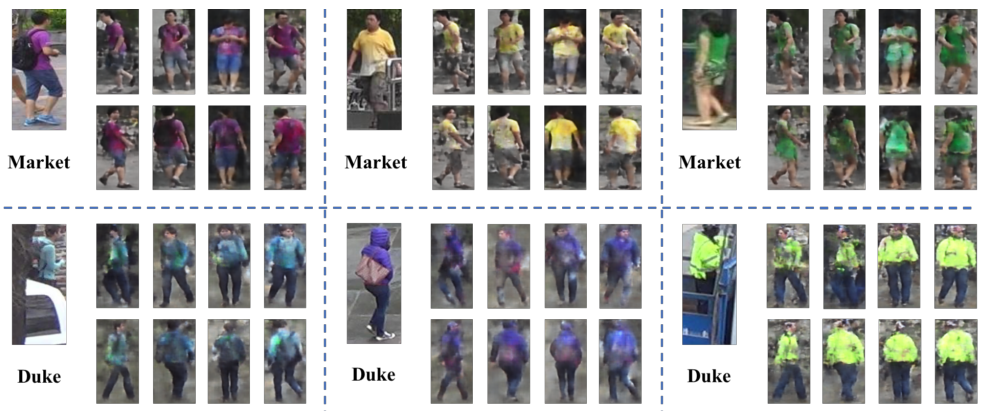
\includegraphics[width=\linewidth,keepaspectratio]{data/kaitibaogao/vis.png}
        \caption{在Market1501和DukeMTMC-reID数据集上生成图片的效果。}
        \label{figure:vis}
    \end{figure}

\section{其他方向}

    目前视觉领域逐渐开始从图片转向了视频,对于再识别而言,两者最大的区别在于询问视频序列具有多张图片。对此,常用的有两种方案:多张query图片多次查询,聚合排序结果;聚合查询图片的特征,然后只进行一次查询。两种方法相比,后者在大规模检索问题中更具实用性和扩展性。因此再识别领域往往借鉴视频动作识别中的想法将多张图片的特征聚合。比如捕捉特征随时间的演化模式、通过在CNN中嵌入三维卷积直接得到视频级别的特征描述。

    累计运动背景网络(Accumulative motion context network, AMOC)\cite{liu2017video}使用视频动作识别中效果最好的双流网络提取空间特征和光流(运动)特征,融合后输入到一个RNN来提取时序特征。其中,由于光流运动信息的提取非常耗时,作者首先训练了一个类似U-Net结构的运动信息网络,输入原始图像序列,前馈网络预测不同尺度的光流图像拼接为最终的预测光流。通过AMOC网络,每个图像序列都能被提取出一个融合了内容信息、运动信息的特征。网络采用了分类损失和对比损失来训练模型。融合了运动信息的序列图像特征能够提高行人重识别的准确度。

    \begin{figure}[!htbp]
        \centering
        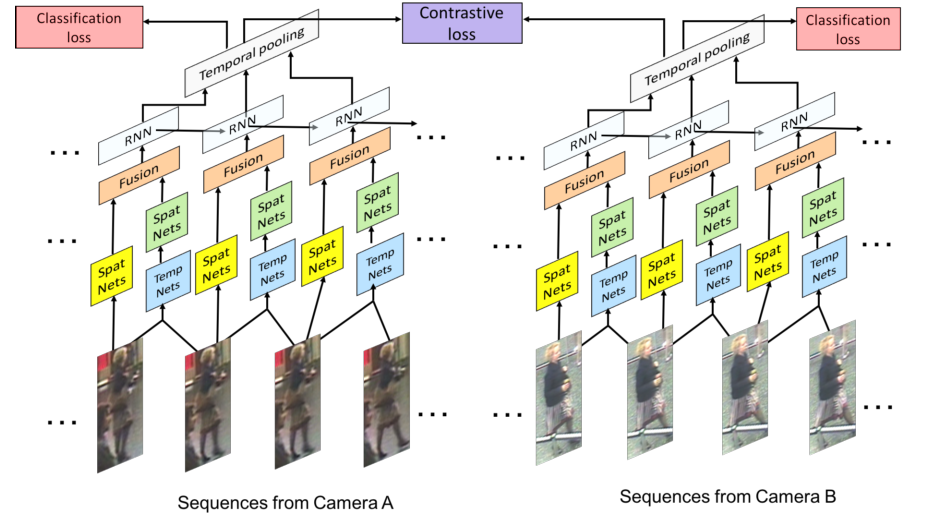
\includegraphics[width=\linewidth,keepaspectratio]{data/kaitibaogao/motion.png}
        \caption{累计运动背景网络结构}
        \label{figure:motion}
    \end{figure}

    另一方面,行人再识别领域的gallery集合中图片数量不断扩大,从传统数据集的100k增长到了500k,开始逐渐迈向大规模检索的现实场景。随着gallery集合的增大,会带来两方面的挑战:性能的下降和速度的下降。
    
    性能方面,由于迷惑项的增加,mAP降幅最大可达7\%。同时为了达到实时的速度,在性能与速度的权衡后,我们往往采用近似最近邻搜索,牺牲一定的精度,导致性能进一步下降。
    
    速度方面,我们非常需要紧凑的特征表达,将一张图片映射到2048维的语义空间和128维的语义空间,在距离矩阵的计算速度上会有巨大差别。从500k到10M的gallery集合,耗时会增加60.7s!于是我们有必要从图像检索领域借鉴想法。但是与图像检索有所区别的是,在训练阶段再识别问题被标注有ID信息,可以作为分类问题;而在测试阶段,再识别问题完全变成了检索问题。除了算法上存在难题,数据集上也还没有达到图像检索的规模。于是近期,悉尼大学的学者将会提出一个具有更多迷惑项、强调检索实时性的行人再识别数据集。


\bibliographystyle{data/gbt7714-2005}
{
\renewcommand{\chapter}[2]{\section*{#2}\addcontentsline{toc}{section}{#2}}
\bibliography{data/kaitibaogao}
}

% 按文章长度需要启用
\ifthenelse{\equal{\zjuside}{T}}{\newpage\mbox{}\thispagestyle{empty}}{}

\chapter{开题报告}

\section{研究开发的背景、意义与目的}

\subsection{背景介绍}

大多数研究者所指的行人再识别目标是跨摄像头识别同一行人[4]。由于姿态、遮挡和背景干扰的存在,再识别任务急需一种强大的特征表示,具有较小的类内间距和较大的类间间距。对此,我们可以从全局特征、局部特征的融合,或者采用全新的训练方式,提升特征的鲁棒性和表达能力。

\subsection{本研究的意义和目的}

从多个角度研究行人再识别,通过广泛阅读行人再识别方面的文献和动手实验,了解行人再识别中真正有用的关键技术。同时也阅读相关领域的论文,行人再识别领域一个很明显的趋势就是不停地从其他领域借鉴新问题和新方法,从人脸验证到图像检索再到信息检索(数据挖掘)。目前人脸验证中的开放环境验证(Open-set Verification)、各种loss函数、使用GAN生成多视角的样本,图像检索中的迷惑图片(Distractor)、大规模信息检索中速度与精度的权衡、可缩减的特征表示[2]、rerank后处理[3]等思路都已经引入行人再识别。信息检索、web搜索中还有一些概念可能还没有引入,比如专家(Expert/Local Model)、社区(Community)。
最后还可以进行的方向包括:结合认知科学中对人类视觉皮层结构的研究成果,提出可变性(Deformable)、动态(Dynamic、Running Time)的模块,提取鲁棒的特征,利用结合IRGAN利用对抗网络挖掘最具竞争力的样本,利用强化学习选择最富有信息的样本,使用记忆网络摒弃所有point2point的方法将set2set的问题[10]真正地解决。
我们也将从行人再识别的各个方面着手,先达到State of the Art的效果,再尝试提出自己的想法。

\section{主要研究开发内容}

\subsection{主要研究内容}

主要研究行人再识别中的起作用的关键技术。包括再识别中的基础技术:siamese network、match network、histogram特征的提取,再识别中起作用的技术:Triplet loss、online hard negative mining、rerank后处理,以及最后在IRGAN、NTM方面继续尝试。

\subsection{技术路线}

从基本方法开始,首先熟悉再识别数据集和任务,然后尝试复现达到最新论文的效果,最后基于之前积累的经验,选择几个最有可能成功的方向,提出想法、进行试验从而能有自己的创新。

\subsection{可行性分析}

分为三个阶段,从熟悉再识别任务,到复现最新方法,再到提出自己的方法,前面两个阶段比较基础,最后一个阶段具有挑战性。
针对发表论文的目标而言,这样的技术路线是否可行?从研究的问题上来说,行人再识别作为新兴的研究方向投稿论文增加,本身课题具有可行性;从使用的方法上来说,我们可能会采用IRGAN、RL、GAN、NTM等方法,或者提出一些基础通用的模型,具有可行性。

针对学习最新方法的目标而言,这样的技术路线是否可行?一方面,我们直接从开源代码、文档、最新论文着手,可以在最短时间内掌握一个最前沿的方向。另一方面,虽然我们没有时间系统阅读Deep Learning、Reinforcement Learning: An Introduction、Element Of Statistics Learning或者学习一些公开课,系统地了解深度学习领域的知识,但是我们会取长补短,仔细选择和仔细阅读相关部分论文,方便撰写论文。具有可行性。

\section{进度安排及预期目标}

\subsection{进度安排} 

\subsubsection{熟悉典型的行人再识别数据集} 

行人再识别中大型的数据集包括CUHK03、Market1501,每个数据集都有自己强调的创新之处,比如CUHK03强调图片数量和行人数目是15年最多的数据集,Market1501在此基础上强调使用DPM检测器,图片质量具有自然场景下应有的噪声与挑战。比较不同的数据集主要可以从行人ID数据、图片数据、训练测试数量、gallery集合大小、数据质量方面衡量。这一阶段,重点掌握各个数据集的共性,准备好各个数据集调用的同一接口,从而方便之后的研究对比实验。

\begin{table}[!htbp]
\centering
\caption{常用数据集的统计特性}
\label{table:dataset}
\begin{tabular}{|l||l|l||l||l|l|}
\hline
cuhk03.combine & \#ids & \#images & market1501 & \#ids & \#images \\ \hline \hline
train & 1267 & 12183 & train &651&11281\\ \hline 
val&100&948&val&100&1655\\ \hline 
trainval&1367&13131&trainval&751&12936\\ \hline 
query&100&965&query&750&16483\\ \hline 
gallery&100&965&gallery&751&19281 \\ \hline
\end{tabular}
\end{table}

当然目前行人再识别领域数据集频出,各种新的任务也不断出现。传统的CUHK01、VIPeR通常只在弱监督、迁移学习中会被研究和使用。视频ReID任务常常使用PRID 2011,iLIDS-VID和MARS。为了衡量每帧图片质量,Sensetime新推出了Labeled Pedestrian in the Wild (LPW)数据集,其中包含7,694个tracklets,超过590,000个图片。为了衡量现实场景下行人搜索任务的性能,悉尼大学的Zheng Liang提出了PRW数据集。为了研究迁移学习,比现有数据集规模再大3.5倍的MSMT17即将开源,该数据集在时空跨度、行人多样性、背景干扰方面的挑战更大。如果有余力,也可以整理一下这方面的数据接口,有助于将来进行Ablation Study。

\subsubsection{广泛阅读文献,熟悉典型的行人再识别方法}

使用CNN做行人再识别的典型方法包括:改进的行人再识别(ImprovedReID)、基于深度语义特征的行人再识别(DCSL)、基于行人局部特征的行人再识别(Part-reid)。
从这些方面的论文着手,了解以前和现在的研究者对行人再识别常用方法存在怎么样的理解、分类甚至偏见。比如悉尼大学的Zheng Liang观察到当每个ID的训练样本达到10张以上时,基于identification方法(IDE,identity discriminative embedding)的模型能很轻松地实现高准确率,而基于Siamese模型的Verification方法,每次只能看见两个样本判断相似与否,难以完全利用所有ID的标注信息。因而该组的学者后续提出的方法的baseline都是IDE模型。这种方法简单有效,但是该组学者没有探索通过挖掘富有信息的样本尽可能利用所有ID标注信息,提升模型泛化能力的方法。因而,我们需要广泛阅读世界各地研究者对再识别的见解,获得全方位的了解。

\subsubsection{通过实验熟悉行人再识别方法,复现最新工作}

TriHard、Part-reid等方法都有开源代码,我们会基于这些工作进行实验,复现最新工作的效果。第一步,通过实验,理解这些方法为什么能起作用,存在什么缺点。
现有模型往往在较小随机选择的训练集子集上达到近乎完美的效果(cmc-1为99\%),但是在测试集上泛化能力不佳(cmc-1为80\%~85\%)。但是事实上,如果使用整个训练集合而非子集合来测试模型的能力,我们发现mAP会下降3.4\%。这说明:一方面,训练集合存在噪声——标注错误,异常数据(Outlier);另一方面,训练集中还存在许多富有信息的样本,在随机选择的过程中被忽略。TriHard的出发点就在于在一个batch里在线地挖掘富有信息的样本。但是这一工作其实具有一定的局限性,比如是否每一个anchor样本都需要寻找对应的难样本、寻找几个。当一个随机选择的batch无法提供更多的信息时,是否需要通过其他方法来寻找最富有信息量的样本。

\begin{figure}[!htbp]
    \centering
    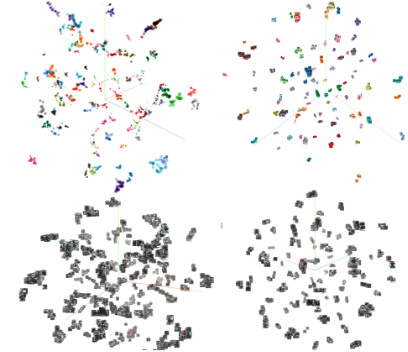
\includegraphics[width=.5\linewidth,keepaspectratio]{data/kaitibaogao/vis2.png}
    \caption{测试集(左图)与训练集合的子集(右图)特征降维可视化。}
    \label{figure:vis2}
\end{figure}

我们也会尝试将在线难样本挖掘用于含有匹配网络的双孪模型。含有匹配网络的双孪模型增大对齐能力的同时也增大了计算量。在这种模型上实现在线难样本挖掘只需要多进行128*128次前向计算(增加1.6s/iter左右的时间),选择最富有信息的样本对即可。这类模型的优点在于可学习的匹配函数,摆脱了欧氏距离的缺点。我们知道目前含有匹配网络的双孪模型较好的水平为80\%(在CUHK03上,cmc-1指标),我们有信心使用在线难样本挖掘将他提升到85.43\%。而用了在线难样本挖掘的三元损失模型(TriHard)只有85\%。因此如果进一步在损失函数、模型结构上扩展,我们也许有机会达到更高的水平。如果按着这一研究方向进行,我们尝试引入一些非线性模型的想法。

在局部特征与全局特征的融合方面,我们会尝试使用Part-reid方法。使用时注意观察TriHard中提到的注意事项会有怎样的影响。比如激活函数的使用,ReLU,L2 Normalize,Sigmoid函数究竟该不该用、用在哪里。小心一些不合理的设置,比如BatchNorm之前和之后同时使用ReLU函数,当模型变得复杂时,很容易出现这些简单的错误。这时候不能归咎于方法不起作用,而应该通过单元测试、输出中间变量可视化等方式找到错误。同时这也有助于我们了解模型的特点和优缺点。

\begin{figure}[!htbp]
    \centering
    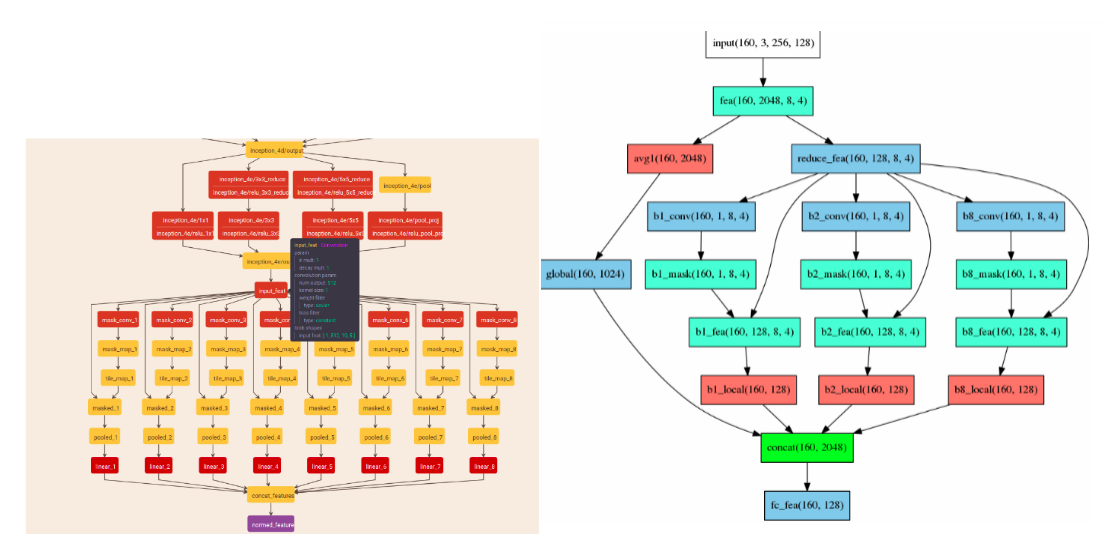
\includegraphics[width=\linewidth,keepaspectratio]{data/kaitibaogao/vis3.png}
    \caption{Part-reid的网络结构,左图:论文中的使用的结构。右图:我们计划实现的版本}
    \label{figure:vis3}
\end{figure}

\subsubsection{提出我们的方法}

我们将在观察到的现象的基础上,提出我们的方法。虽然想法很重要,决定了一篇文章是否有影响力,但是目前很难下定论,什么样的想法能够起作用。
按照最初课题的方向,我们可以从GAN、Video的角度着手,比如使用IRGAN选择富有信息的样本,GAN的训练比较困难会遇到训练崩溃的情况,对此一定要耐心调试、多吸取前人的经验。针对Video数据,一方面可以提取时序特征,作为行人的描述子;另一方面,可以将问题转化为multi-shot的问题,考虑每帧图片的质量的基础上进行特征融合。
同时也可以在其他方面着手,比如目前的reid研究都强行将set2set的问题[1]转化为point2point,无论训练还是测试都只比较两张图片的相似度。这才让rerank有机可乘。可以尝试结合NTM将rerank利用上下文信息的步骤端到端地结合到网络中,从而在一定意义上实现自动的single-shot到multi-shot的转换。同时我们也会在选择样本、特征提取、基础卷积模块的设计上着手,选择最有效果的方向深入研究。

\subsection{预期目标}

\begin{enumerate} 
\item 熟悉典型的行人再识别数据集:编写统一的调用接口。
\item 广泛阅读文献,熟悉典型的行人再识别方法:全面了解行人再识别问题和解决方法。
\item 通过实验熟悉行人再识别方法,复现最新工作:达到前沿方法的效果。
\item 提出我们的方法:通过对模型的了解,尝试不同方法,提出新的想法。
\end{enumerate}

{
% \renewcommand{\section}[2]{\section*{#2}\addcontentsline{toc}{section}{#2}}
\section{参考文献}
}

\begin{itemize}
\item [{[}1{]}] Y. Liu, J.Yan, andW. Ouyang. Quality aware network for set to set recognition. arXiv preprint arXiv:1704.03373, 2017
\item [{[}2{]}] X. Liu, H. Zhao, M. Tian, L. Sheng, J. Shao, S. Yi, J. Yan, and X. Wang. Hydraplus-net: Attentive deep features for pedestrian analysis. 2017.
\item [{[}3{]}] Zhong, Z., Zheng, L., Cao, D., \& Li, S. (2017). Re-ranking Person Re-identification with k-reciprocal Encoding. \url{http://arxiv.org/abs/1701.08398}
\item [{[}4{]}] Zheng, L., Yang, Y., \& Hauptmann, A. G. (2016). Person Re-identification: Past, Present and Future. \url{http://arxiv.org/abs/1610.02984}
\item [{[}5{]}] Wang, J., Wang, B., Zhang, P., \& Zhang, D. (2017). IRGAN : A Minimax Game for Unifying Generative and Discriminative Information Retrieval Models.
\end{itemize}


% 按文章长度需要启用
\ifthenelse{\equal{\zjuside}{T}}{\newpage\mbox{}\thispagestyle{empty}}{}

}

{
	\pagestyle{waiwenfanyi}
	\makeatletter
	\let\ps@plain\ps@waiwenfanyi
	\makeatother
	% \setcounter{page}{1}

	% \renewcommand{\addcontentsline}[3]{}

	% !TeX root = ../main.tex

\chapter{文献翻译}

 {
  \setlength{\parindent}{0em}

  文献原文:

  Zhang X, Luo H, Fan X, et al. AlignedReID: Surpassing Human-Level Performance in Person Re-Identification, 2017. \par

 }

\vspace{2em}

{
	\renewcommand{\cleardoublepage}{}
	\renewcommand{\clearpage}{}
	\titleformat{\chapter}[block]{\sanhao\songti\bfseries\filcenter}{}{0em}{}{}
	\chapter*{对齐再识别:超越人类的表现}
}

\section*{摘要}

在这篇论文中,我们提出了一种全新的方法,叫做对齐再识别。最终部署时只使用全局特征,全局特征的鉴别能力是通过与局部特征的共同学习获得的。在共同学习的过程中,局部特征通过计算最短路径对齐和匹配不同人体区域,不需要额外的监督信息。在学习完成之后,我们只使用全局特征计算图像的相似度,进行检索。我们的方法在Market1501数据集上获得了94.0\%的rank-1准确率,在CUHK03上获得了96.1\%的rank-1准确率,均比目前最好的方法提升了很多。我们也评估了人类所能达到的极限,发现我们的方法首次在两个公开数据集上超过了人类表现!

\section{介绍}

行人再识别,是计算机视觉中的一个子任务,目标是在不同的时空鉴别出目标行人。他应用广泛,从跨摄像头跟踪,到销售商店客流量分析,均可发挥巨大作用。同很多视觉任务一样,再识别的难点也在于视角,光照的变化和遮挡的存在。
传统的方法通常在底层特征上着力。但自从深度学习复兴之后,卷积神经网络成为了这一难题的主流方法,通过端到端的特征学习,以及丰富的度量学习损失函数设计(比如对比损失,三元损失,四元损失和难样本挖掘三元损失),这一方法达到了前所未有的准确率。
很多卷积神经网络的方法仅仅考虑学习全局特征,而忽略了行人的空间结构。这些方法主要有以下缺点:
\begin{enumerate}
	\item 不准确的行人检测会影响特征学习。
	\item 行人被遮挡时,全局特征会引入无关的背景信息。
	\item 视角变化和非刚性物体的形变使度量学习更加困难。
	\item 外观相似但并非同一人的情况大量存在,这时候需要突出局部特征才能鉴别出这类行人。
\end{enumerate}
为了解决上述问题,近期的一些工作在划分人体区域学习局部特征上着手,但是仍然无法解决检测不准确、姿态变化、遮挡等难题。也有研究者从姿态估计着手,但是这种方法需要额外的监督信息,同时在姿态估计的步骤中往往更容易发生错误。
在本文中,我们提出了一种全新的对齐再识别的方法,虽然也是学习全局特征。但是在学习的过程中使用局部特征对齐协同学习,不需要额外的监督信息或者显式的姿态估计。在学习阶段,我们有两条支路分别学习局部特征和全局特征。在局部特征支路,我们引入了最短路径损失。在部署使用阶段,我们只使用全局特征。因为我们发现只使用全局特征已经和多种特征融合的效果同样好!这从另一方面说明,在协同训练的过程中,局部特征帮助全局特征变得更有鉴别能力。同时简洁的全局特征使得我们的方法便于部署到大尺度行人再识别系统中。

\section{方法}

\subsection{对齐再识别}

对于每张输入图片,我们使用Resnet50提取特征,得到2048X7X7的特征图,然后使用全局池化得到2048维的全局特征。对于局部特征我们首先使用使用垂直方向的池化得到2048X7的特征图,然后使用动态匹配局部区域,得到最小距离,作为局部特征之间的距离度量。这样的特征提取方式隐含着人在图片中通常直立的假设。
给定两幅图片的局部特征,在我们的实验中H为7,即行人从头到脚被分为7个部分。我们首先计算两两之间的距离矩阵:
\begin{equation} {d_{i,j}} = \frac{{{e^{\|{f_i} - {g_j}\|{_2}}} - 1}}{{{e^{\|{f_i} - {g_j}\|{_2}}} + 1}}\qquad i,j \in 1,2,3, \cdots ,H \end{equation}

采用这样形式的变换的原因是:改距离可以归一化到[0,1]之间。然后定义局部特征时间的距离为距离矩阵D中,从(1,1)到(H,H)之间的最短路径。改最短路可以由动态规划计算得到。如图1所示,图像A和图像B是同一行人的不同视角的图片。身体不同部分的对齐,比如图A的第一部分和图B的第4部分,在最短路径的第一个转折中体现出来。同时,也存在一些不对应部分的对齐,比如图A的第一部分和图B的第一部分。我们认为,不对应部分的对齐是有助于维护垂直对齐的顺序的。不对应部分有着更大的L2距离,梯度更接近于0,英尺这些对齐在最短路中贡献可以忽略。因此最短路的总距离主要由对应部分的对齐决定。

\begin{figure}
	\centering
	\captionsetup{width=.88\linewidth}
	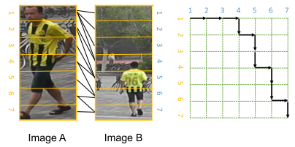
\includegraphics[width=.6\linewidth,keepaspectratio]{data/waiwenfanyi/placeholder.png}
	\caption{\kaiti 图像A和图像B是同一行人的不同视角的图片。身体不同部分的对齐,比如图A的第一部分和图B的第4部分,在最短路径的第一个转折中体现出来。}
	\label{figure:placeholder}
\end{figure}

全局和局部特征共同定义了图像在学习阶段的距离。我们选择TriHard损失作为度量损失函数。对于每一个样本,我们会根据全局特征之间的距离选取最有竞争力的样本对,获得3元组。而三元组的损失则是根据全局特征距离和局部特征距离共同计算的。这样做的原因出于两点考虑:1. 全局距离的计算更加快;2. 我们观察到使用全局距离和局部距离作为难样本挖掘的手段,没有很大的差别。

\subsection{Mutual Learning应用于度量学习}

我们将mutual learning应用于对齐再识别中,来进一步提升效果。在知识蒸馏一文中,作者使用小的学生网络学习大的教师网络中的知识。他的工作用于分类任务中,与他的工作不同,我们采用矩阵级别的均方误差作为新提出的相互学习损失,用于度量学习的任务中。

总体的损失由度量损失、分类损失、分类相互学习损失和度量相互学习损失构成。其中,度量损失是由局部和全局特征距离共同决定的,但是度量相互损失仅由全局特征距离决定。
下面介绍度量相互损失的实现:给定一个batch的图片,可以使用全局特征计算出距离矩阵。使用ResNet50和Resnet50-Xception作为基础骨架模型,得到两个不同的学生模型。使用距离矩阵的均方误差作为损失函数,使得两个学生相互学习。在实践中,我们发现使用停止梯度的操作可以加快收敛。即停止Resnet50学生网络的梯度更新,将其作为常数,使得Resnet50-Xception学生逼近Resnet50,以及用相同的方式让Resnet50逼近Resnet50-Xception。

\section{实验}

\subsection{数据集}

Market1501数据集包含32668张图像,1501个行人,6个摄像视角。训练集中有750个行人,测试集中有751个行人。与提出数据集的作者相同,我们也将mAP作为我们的指标的一种。

CUHK03包含13164张图片,1360个行人,他同时提供了DPM检测器检测的行人和手工标注的行人。

MARS数据集是Market1501的扩展版本,所有的行人都是自动检测的。因此可能包含一些虚警增加难度,同时每个ID可能包含多余1个候选答案。他包含20478个tracklet和1261个行人,6个拍摄视角。

CUHK-SYSU是一个大尺度行人搜索的数据集,包含18184张图片,每张图中含有多个行人,共计99809个行人检测框,8432个行人。

注意我们使用全部数据集的样例训练单个模型,对于MARS、CUHK-SYSU和Market1501数据集我们使用官方的训练和评估协议。但是在CUHK03上,由于我们使用了全部benchmark的数据集训练了一个模型,和官方的测试方式(随机划分数据集为训练集和测试集,测试包含100个行人,重复20次)有些不同。因此,我们仅仅随机划分数据集一次,训练集与其他数据集的训练集一同作为整个模型的训练集,将测试集作为CUHK03上衡量CUHK03数据集性能的测试集。由于我们划分的测试集含有200个行人,可以认为这个评估协议比原始的协议更具有挑战性。

\subsection{实现细节}

我们使用Resnet50和Resnet50-Xception制品为基础模型。输入图片缩放到224X224。数据增强使用随机水平翻转和随机截取。TriHard损失的margin设为0.3,mini-batch设为128,在一个batch中确保每个id的图片有4张。每个epoch包含2000个mini-batch。我们采用adam优化器,初始学习率设为0.001,在第80和第160个epoch时,衰减0.1训练至收敛。
对于对偶学习,相互分类损失的权重设为0.01,相互度量损失的权重设为0.001,使用adam优化器。初始学习率设为0.0003,分别在60和120epochs时衰减到0.0001和0.00001。

\subsection{对齐再识别的优点}

我们首先定性分析对齐的效果。在图2的(a)中,由于右边行人的检测不准确,两张原始图片原本无法对齐。对齐再识别算法将左边第一部分和右边的上上个部分匹配在一起,实现了对齐。在(d)中两个行人外观相似,但属于不同id,右边行人衣服上的标志找在左边找不到相似的部分,因此最短路中对应部分的路径也变得更长。

\begin{figure}
	\centering
	\captionsetup{width=.88\linewidth}
	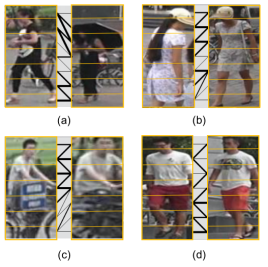
\includegraphics[width=.45\linewidth,keepaspectratio]{data/waiwenfanyi/fig2.png}
	\caption{\kaiti 黑色线条表示两个新人局部的对齐:加粗表示对最短路贡献大。在(a-c)中行人有着相同的id,而在(d)中行人有着不同的id。}
	\label{figure:fig2}
\end{figure}

然后我们将对齐再识别与基准模型对比。基准模型没有使用局部特征支路。两个结果使用相同的网络和训练参数设置。我们观察到对齐再识别方法能提升3.5\%到6.0\%的rank-1指标和5.0\%到8.4\%的mAP指标。
我们发现将局部特征和全局特征放在一起,rank-1指标只进一步提升了0.3\%到0.5\%,但该方法会变得更加耗时,因此我们推荐只是用全局特征。

\subsection{与其他最新方法比较}

在Market1501数据集上,使用rerank的GLAD达到了89.9\%的rank-1指标和81.1\%的mAP。而我们的对齐再识别在没有使用rerank的情况下就达到了92.6\%的rank-1指标和82.3\%的mAP。如果使用rerank,则进一步提升到94\%和91.2\%

在CUHK03数据集上,在不使用rerank的情况下HydraPlus-Net获得了91.8\%的rank1,而我们的对齐再识别为91.9\%。再次强调,我们的测试候选集为200张,我们的测试协议更加困难。同时在使用rerank的情况下,我们的方法获得了96.1\%的rank-1。

\begin{figure}
	\centering
	\captionsetup{width=.88\linewidth}
	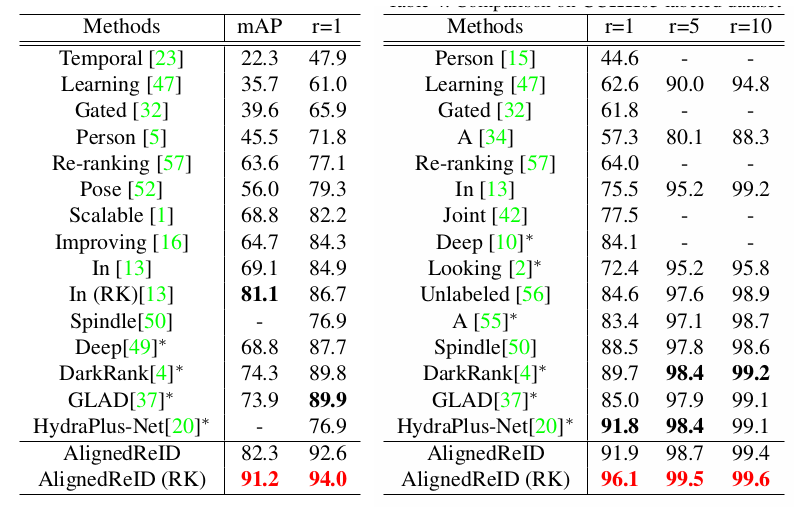
\includegraphics[width=.85\linewidth,keepaspectratio]{data/waiwenfanyi/compare.png}
	\caption{\kaiti 左图:在Market1501数据集上的性能比较,右图:在CUHK03数据集上的性能比较}
	\label{figure:compare}
\end{figure}

\subsection{总结}
在这篇文章中,我们阐明了隐式局部特征对齐对提升全局特征学习的巨大作用。这一惊奇的结果给予了我们重要启发:1). 端到端的学习需要结构先验,否则就是盲学。2). 我们的方法尽管在Market1501和cuhk03数据集上超过了人类的表现,但是在验证集中也会犯一些低级错误。可见机器想要在更广泛的领域战胜人类仍然有很长的路要走。

% \begin{figure}
% 	\centering
% 	\captionsetup{width=.88\linewidth}
% 	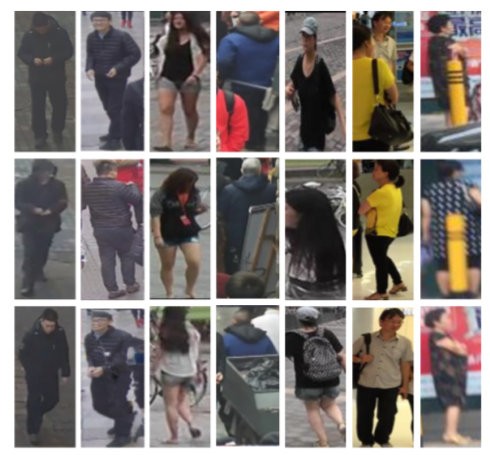
\includegraphics[width=.6\linewidth,keepaspectratio]{data/waiwenfanyi/bad.png}
% 	\caption{\kaiti 在验证集中发现的一些低级错误}
% 	\label{figure:bad}
% \end{figure}

}

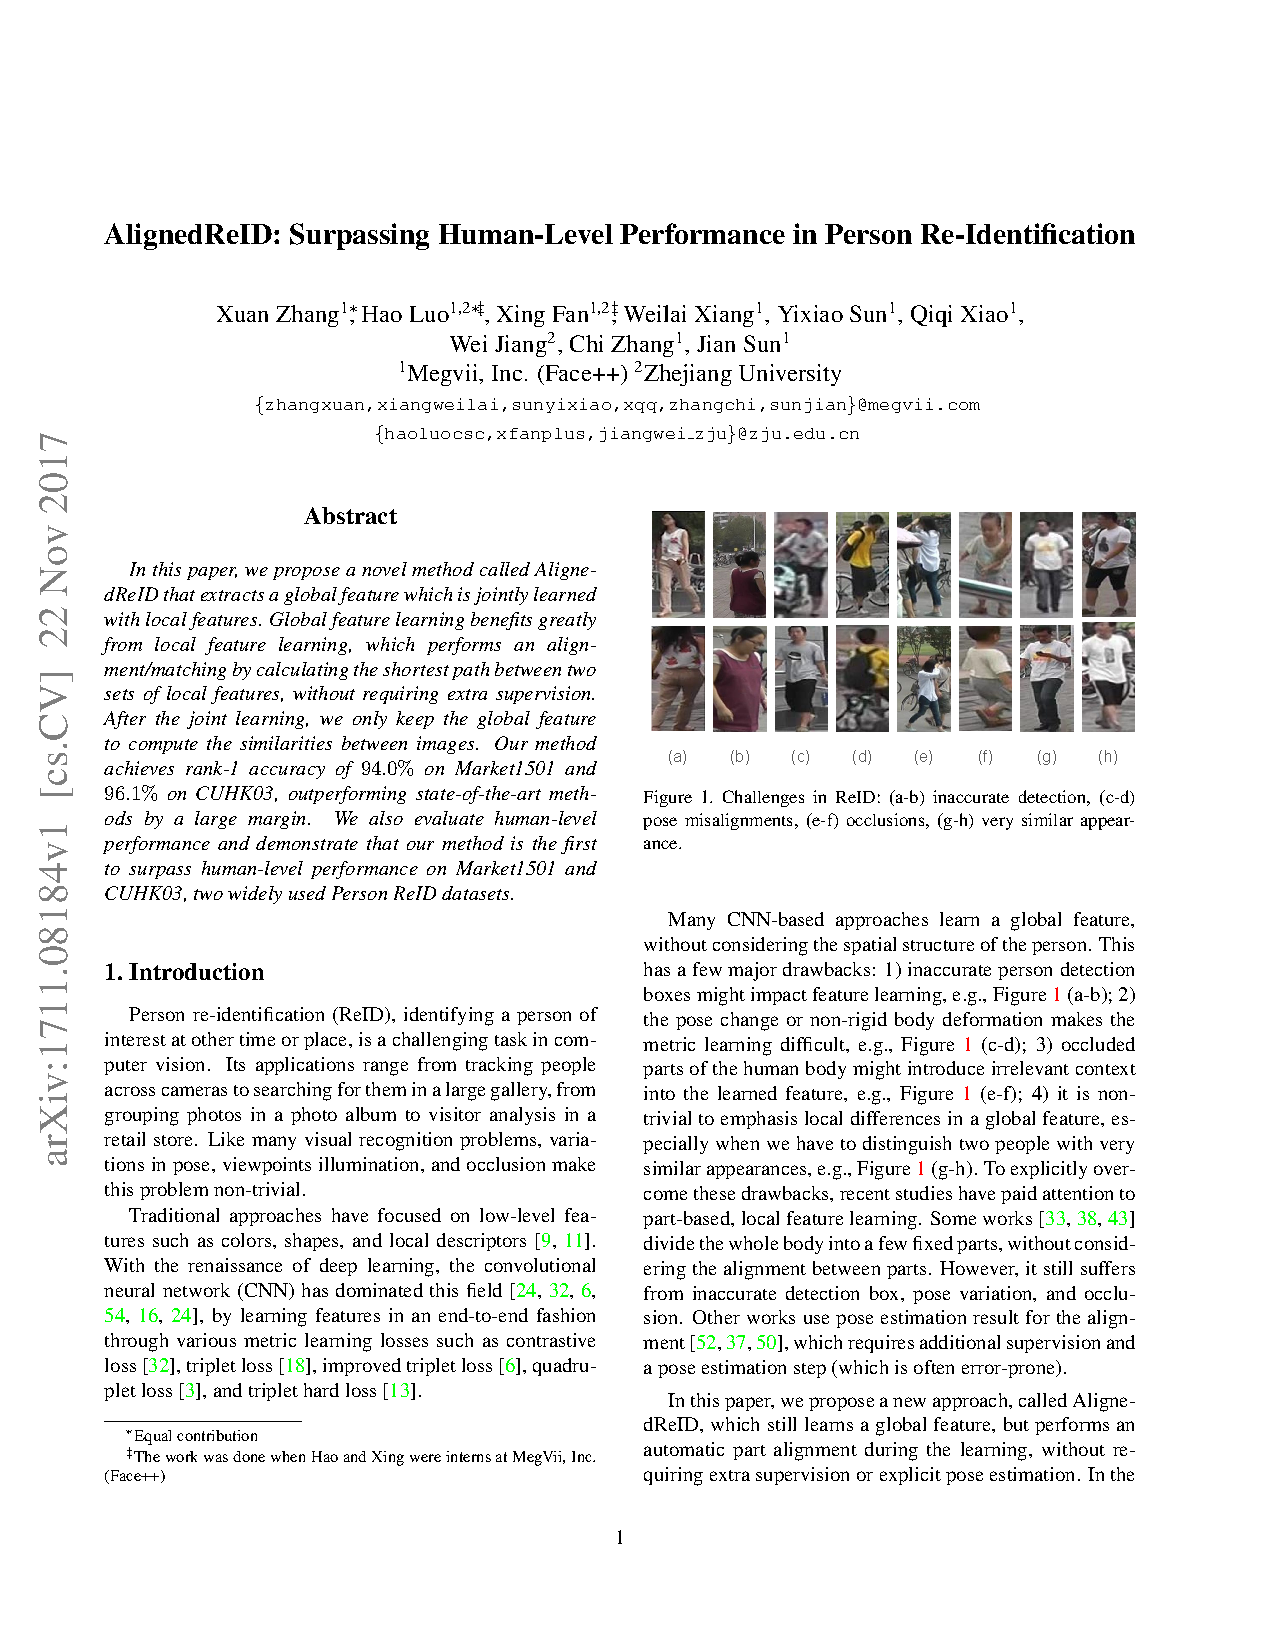
\includepdf[scale=0.8,pages=1,pagecommand=\chapter{外文原文}]{data/waiwenyuanwen.pdf}
\includepdf[pages=2-]{data/waiwenyuanwen.pdf}
% 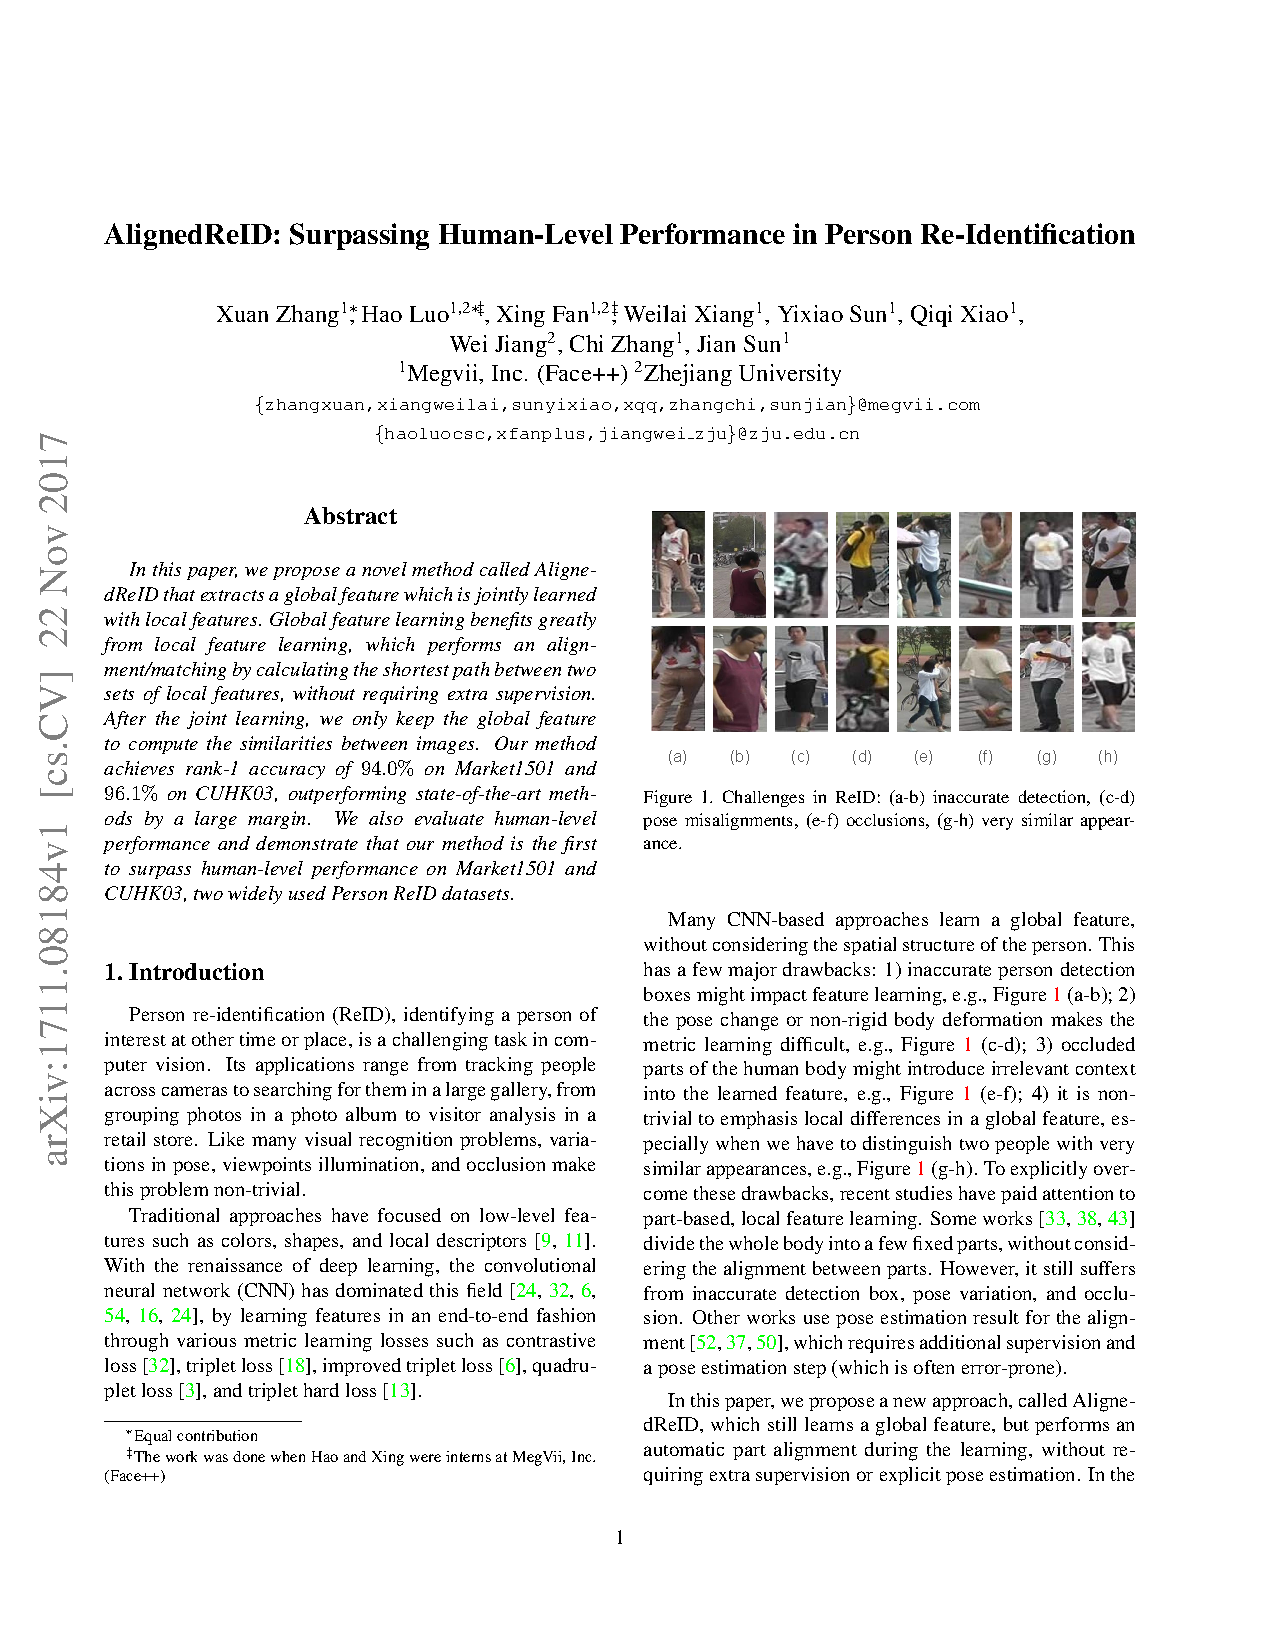
\includepdf{data/waiwenyuanwen.pdf}
\backmatter

{  % !TeX root = ../main.tex

\thispagestyle{empty}

{
	\setlength{\parindent}{0em}
	\renewcommand{\baselinestretch}{2}

	{
		\stfangsong\sanhao\bfseries
		\centering
		毕业设计文献综述和开题报告的考核 \par
	}

	{
		{\kaiti\sihao\bfseries
				一、对文献综述、外文翻译和开题报告评语及成绩评定:}

			{\songti\sihao \bfseries
				评语: \\
      }
      
      \vspace{2em}
      
      {\songti \xiaosi 文献综述对国内外研究现状进行了一定的论述。开题报告框架合理,技术路线可行,研究内容和时间节点安排适当,书写规范。文献翻译忠实原文,语句通顺。答辩过程中,叙述清楚,回答问题正确。有一定的创新性。通过开题答辩,同意转入下一阶段的毕业设计。存在问题:进一步完善报告格式美观性。}

		\vspace{12em}

		% {
		%   \renewcommand{\baselinestretch}{1}

		%   \begin{flushright}

		%     \begin{tabular}{|c|c|c|c|}
		%       \hline
		%       成绩比例 & \parbox[c]{3.6em}{\xiaosi 开题报告 \\ 占(20\%) \vspace{0.25em}} & \parbox[c]{3.6em}{\xiaosi 外文翻译 \\ 占(10\%) \vspace{0.25em}} \\
		%       \hline
		%       分值 & & \\
		%       \hline
		%     \end{tabular}

		%     \vspace{2em}

		%     {
		%       \songti\xiaosi\bfseries
		%       导师签名 \; \underline{\hspace{6em}} \\
		%       年 \qquad 月 \qquad 日 \par
		%     }
		%   \end{flushright}
		% }
	}

	\vspace{2em}

	{
		{\songti\sihao\bfseries
		成绩:}

		\vspace{2em}

		{
			\renewcommand{\baselinestretch}{1}
			\songti\sihao
			
\begin{flushleft}
	\begin{tabular}{|c|c|c|c|}
		\hline
		成绩 & \parbox[c]{4em}{\vspace{0.5em}\xiaosi 文献综述                              \\ 占(10\%) \vspace{0.5em}} & \parbox[c]{4em}{\vspace{0.5em}\xiaosi 开题报告 \\ 占(15\%) \vspace{0.5em}} & \parbox[c]{4em}{\vspace{0.5em}\xiaosi 外文翻译 \\ 占(5\%) \vspace{0.5em}} \\
		\hline
		分值 & {\xiaosi 7}                                    & {\xiaosi 12} & {\xiaosi 4} \\
		\hline
	\end{tabular}
\end{flushleft}

\vspace{7em}

\begin{flushright}

	{
		\songti\xiaosi\bfseries
		开题报告答辩小组负责人(签名): \; \underline{\quad 张婷 \quad} \\
		2018 年 3 月 20 日 \par
	}
\end{flushright}
		}
	}

	% \newpage

	% {
	%   \stfangsong\sanhao\bfseries
	%   \centering
	%   毕业设计中期报告考核 \par
	% }

	% {
	%   \songti\sihao\bfseries
	%   导师对中期报告的评语及成绩评定:

	%   \vspace{10em}

	%   {
	%     \renewcommand{\baselinestretch}{1}

	%     \begin{flushright}

	%       \begin{tabular}{|c|c|c|c|}
	%         \hline
	%         成绩比例 & \parbox[c]{3.6em}{\xiaosi 中期报告 \\ 占(10\%) \vspace{0.25em}} \\
	%         \hline
	%         分值 & \\
	%         \hline
	%       \end{tabular}

	%       \vspace{2em}

	%       {
	%         \songti\xiaosi\bfseries
	%         导师签名 \; \underline{\hspace{6em}} \\
	%         年 \qquad 月 \qquad 日 \par
	%       }
	%     \end{flushright}
	%   }
	% }
}
 }

\end{document}
